% What they are, types and characteristics
%	\begin{figure}[tbp]
%		\begin{minipage}[c]{.48\linewidth}
%			\centering
%			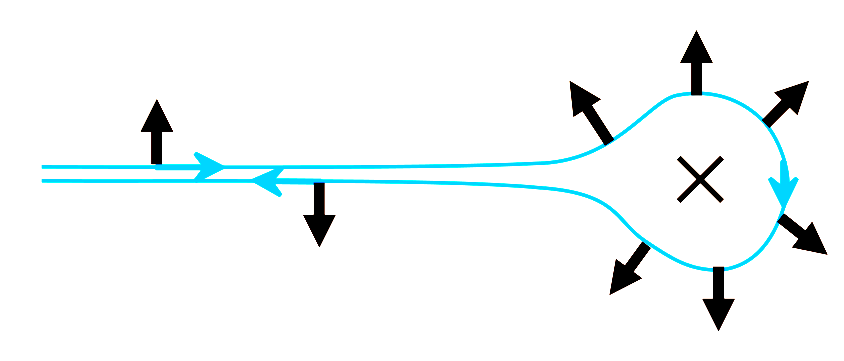
\includegraphics[width=\linewidth]{electron_spin_reflection_1.png}	
%		\end{minipage}
%		\hfill
%		\begin{minipage}[c]{.48\linewidth}
%			\centering
%			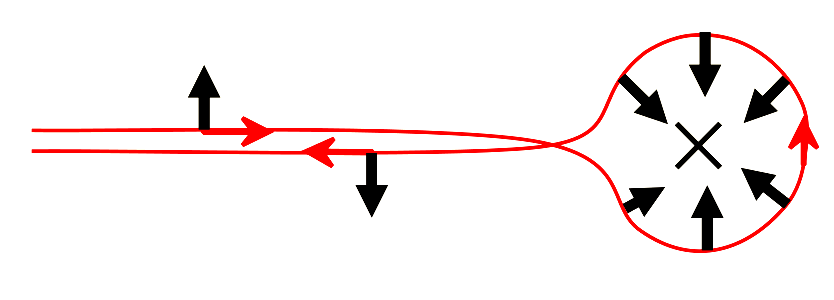
\includegraphics[width=\linewidth]{electron_spin_reflection_2.png}	
%		\end{minipage}
%		\caption{Two different ways of an electron's spin is been reflected off an impurity, which has no magnetic momentum. Both are turning the spin from $\pi$ to $-\pi$ which is a difference of $2\pi$, thus the spins destruct each other and ensure perfect transmission. The time-reversal symmetry is hence guaranteed. (Picture from \cite{topological_insulators}) } \label{electron_spin_reflection}
%	\end{figure}
%	They can be classified by topological order into trivial and non-trivial insulators. The latter ones contain conducting states at the surface.  

%	Insulators in general are in lack of freely flowing electric charges so that no current flows under influence of an electric field. But under sufficiently large voltage, an insulator still becomes conductive by tearing the electrons away from the atoms. Experimentally this means, that they have a higher resistivity than semi-conductors and conductors. 
%
%
%	The concept of topological insulators (TIs) was first predicted in two dimensional space, more specific, the predictions are related to quantum spin Hall (QSH) edge states in graphene band structures discovered by Kane and Mele \cite{Kane_Mele1} by applying spin-orbit coupling (SOC) (see subsection \ref{chapter_soc}). The SOC including gave rise to a gap opening where graphene normally has no gap in its Dirac band structure. But this gapping is different than the ones of normal semi-conductors. Namely the band ordering is inverted and this inversion is different for an opposite spin. This comes from the spin-momentum locking, which means, spin and momentum remain perpendicular to each other. Additionally prevents backscattering for the QSH edge states. If a flowing electron is back scattered by a non-magnetic impurity, it will act destructively on the incoming one. This is illustrated in figure \ref{electron_spin_reflection}. The physical designation the two QSH edge states which are moving in opposite direction is a Kramers douple, and the phenomenon of prohibited backscattering is due to the protection of the time-reversal symmetry. 
%	That symmetry can be broken by e.g. an magnetic impurity which opens a gap without QSH edge states. 
%	
%	Since this means that material with that property differs from other insulators by their topological order, Kane and Mele \cite{Kane_Mele2} introduced the topological invariant $\Z_2$, which can be broken down to two simple integers 0 and 1, trivial and non-trivial TI. This gave rise to the name 'topological insulator', where either there are QSH edge states protected by time-reversal symmetry or the time-reversal symmetry is broken and there is a band gap with no QSH states.
	Originally, materials were named conductors if, by applying an electric field or an insulator, small electric currents start to flow as a reaction to the external field. 
	
	But 2005 Kane and Mele \cite{Kane_Mele1} discovered that apart from the insulators, the conductors and the semiconductors, there is an other class of material: the so-called topological insulator, which acts like an insulator in the inner part (bulk) but is conductive at the surface. 
	Additionally the surface states of these topological insulators are special in comparison with normal surfaces since they are symmetry protected by time-reversal symmetry and because of their band structure. 
	
	From a practical point of view topological insulators arise by combination of spin-orbit interactions, which itself provide spin-momentum locking and band inversion, and closed energy bands. Because of the spin-momentum locking, backscattering is not possible for surface states as long as time-reversal symmetry is preserved. The reason is, that the spin can not change while the momentum doesn't. 
	The band inversion is the origin for the characteristic Dirac cones of the surface states which lie between the band gap.
	A sketch of one Dirac cone on the surface is illustrated in figure \ref{band_structure_top_insulator}.
	Note that the surface states cannot be removed by modification, i.e. by passivation or disorder, as long as time-reversal symmetry is preserved. 
	
	In 2D a topological insulator possesses 1D edge channels which are counter propagating and spin polarized \cite{Kane_Mele2}. They are known as quantum spin Hall edge states and were first predicted in graphene \cite{Kane_Mele2} but later were found in HgTe quantum wells \cite{Bernevig}. 
	
	Quantum wells have non-trivial topological surface states under a certain critical thickness but become trivial insulators as soon as they pass this critical thickness. 
	\begin{figure}[b!]
		\centering
		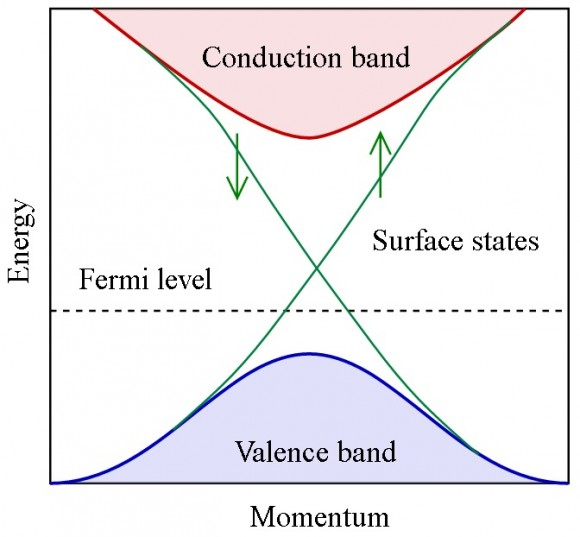
\includegraphics[width=0.4\linewidth]{andere_bilder/band_structure_top_insulator.jpg}
		\caption{%Band structure near the Fermi level for a topological insulator. Due to spin-momentum locking, the surface states are protected. The electrons can flow so well, that the surface is conductive
			Sketch of band structure of a topological insulator near the Fermi level (dashed lines). In blue: valence band, in red: conduction band, in green: the surface states with nearly linear dispersion close to the Fermi level. Each branch of the Dirac cone have opposite spin polarization in respect to the other branch. 
			(Picture from \cite{wiki_top_ins})} \label{band_structure_top_insulator}
	\end{figure}
	
	The prediction was closely followed by the generalization of the concept of topological insulators on to 3D. 
	In this dimension there are two different kinds of topological insulators which are defined by the band structure characteristics: There are strong topological insulators which have an odd number of Dirac cones in the bulk band structure and there are weak ones with an even number of those Dirac cones. 
	
	HgTe, which is the material we consider in this thesis, is also a 3D topological insulator under certain circumstances. In general it is a semi metal, but under applied strain its $\Gamma_6$ and $\Gamma_8$ bands close up at the Fermi level \cite{textbook_ti}. This was confirmed by experimental ARPRES and tranport measurements.
	
	An interesting question is what happens to the band structure and the topological properties by applying strains in one direction. This question will be partly answered in the following sections.
%	But for graphene, the band gap predicted is too small and shows up just at very low temperature, which makes it impossible to observe with todays technical equipment.  
%	In contrast these properties were found in HgTe quantum wells. 
%	A quantum well is a potential with only discrete energy values. Experimentally this can be obtained by stealing one degree of freedom from original free movers in three dimensional space, so that they just can move in a plane.
%	For HgTe this is obtained by sandwiching it between a material that has larger band gaps, which in addition always needs to be thicker than the HgTe in the middle. 
%
%	Above the critical thickness $6.5 \,\unit{nm}$, the HgTe quantum well develops topologically non-trivial states, i.e. the QSH states, with reversed conduction and valence band. Below that thickness the bands are normally ordered and it has topologically trivial states, that is to say a normal band gap. 
%	
%	The concept of topologically protected states can be transfered to three dimensional systems with four different topological $\Z_2$ invariants (Moore and Balents \cite{Moore}). Fu, Kane and Mele \cite{Fu_Kane_Mele} categorized the non-trivial topological states into weak and strong ones, according to their robustness against disorder. HgTe is a strong one and thus develops surface states with an odd number of Dirac cones while the bulk, the inner part of the metal, is insulating. 
%	
%	Those surface states are very similar to the QSH edge states, where the latter are one dimensional states in two dimensional space and the earlier are two dimensional states in three dimensional space. The Dirac cones which live in the $\kk$-space, are those surface states where the spin rotates with $\kk$ around the Fermi surface as long as time-reversal symmetry is conserved. The manifestation of the a Dirac cone in the band structure looks as shown in figure \ref{band_structure_top_insulator}.  
%	The simplest case is a single Dirac cone, which is the case for HgTe. 

%	The topological insulators are solid materials made out of heavy elements which are insulating at the inner part but conducting at the surface. Additionally they have surface states which are protected by particle number conservation and time-reversal symmetry. 
%	
%	The characteristic band structure of a topological insulator is illustrated in figure \ref{band_structure_top_insulator}. The surface states colored in green arise because of the band inversion of the valence band and the conduction band which is induced by the spin momentum locking. And this again arises of to the strong spin-orbit coupling (SOC) which are induced by the relativistic effects of heavy elements.
%	
%%	This means the spin and the momentum are always normal and thus the electrons can just go those two ways. 
%	This surface state structure is called a Dirac cone and is additionally protected by time-reversal symmetry.
%	This means, if an electron is reflected by an non magnetic impurity, the spin gets reflected by a rotation of $2 \pi$, so that it can act destructively on the incoming electron, see figure \ref{electron_spin_reflection} for illustration.
%	In contrast, true magnetic impurities can destroy those surface states because the rotation would be in a way, that the reflected electrons are no longer destructing the incoming ones.
%	 
%	Because there are two ways of reflecting destructively, see blue and red lines in the figure, there are two ways of conserving the time-reversal symmetry. 
%	\\\\	
%	%		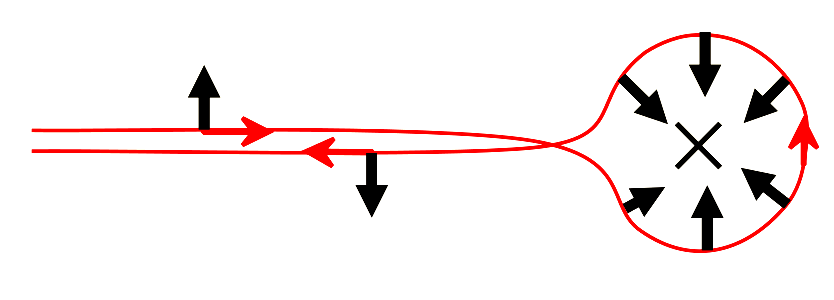
\includegraphics[width=\paperwidth]{electron_spin_reflection_2.png}
%	The underlying ways of defining the topological insulators are the noninteracting topological band theory \cite{Kane_Mele1} \cite{Moore} \cite{Roy}, which relies on the quantum spin Hall effect and the topological field theory \cite{Hughes_Zhang} \cite{Qi}, where the effective Maxwell action which describes the insulator's electron response, is rewritten in a way, that it no longer depends on the geometry of the insulator, but on it's topology.
%%	\begin{equation} \label{Maxwell_action}
%%		S_{\text{Maxwell}} = \frac{1}{16 \pi} \int \diff^3 x \,\diff t 
%%		\left(\epsilon \vec{E}^2 - \frac{1}{\mu} \vec{B}^2\right)
%%	\end{equation}
%%	with $\epsilon$ being the electric permittivity and $\mu$ the magnetic permeability, can be rewritten in dependence on a parameter $\theta$ \begin{equation}\label{topological_action}
%%		 S_\theta = \frac{\theta \alpha}{4 \pi^2} \int \diff^3 x\, \diff t \vec{E} \cdot \vec{B}
%%	\end{equation} 
%%	with $\alpha= e^2/\hbar c$, which only can accept two different values for preserving time-reversal symmetry, $\theta = 0$ or $\theta =\pi$. This implicates, that this action no longer depends on geometry, but on the topology. 
%	
%	Both ways of defining the types of topological insulators are leading to the so called $Z_2$ classification similar to the genus in topology. This means, every insulator of this kind can be categorized by an explicit topological invariant that can only give binary values of 0 and 1. 

%%% Local Variables:
%%% mode: latex
%%% TeX-master: "main_BA2.0"
%%% End: